\chapter[Overview]{Overview} \label{ch:intro}
%
%?There are those who love to get dirty and fix things. They drink coffee at dawn, beer after work. And those who stay clean, just appreciate things. At breakfast they have milk and juice at night. There are those who do both, they drink tea.? 
%? Gary Snyder
%
%?Nature is not a place to visit. It is home.? 
%? Gary Snyder
%
%
%?Three-fourths of philosophy and literature is the talk of people trying to convince themselves that they really like the cage they were tricked into entering.? 
%? Gary Snyder
%
%
%?With no surroundings there can be no path, and with no path one cannot become free.? 
%? Gary Snyder, Practice of the Wild
%
\vspace{-16pt} \begin{chapquote}{Gary Snyder quoting Ezra Pound para-phrasing Lu Ji} \singlespacing ``When making an axe handle, the pattern is near at hand.'' 
 \end{chapquote} \vspace{-8pt}
\noindent\makebox[\linewidth]{\rule{0.5\textwidth}{0.5pt}} \vspace{1pt}
%1)  Introduce the concept of gravitational radiation and its importance.
%	a) what are GWs
%	b) What are the expected sources of GWs
%	c) How are GWs detected - list of experiments and their sensitivity (Figure?)
%2) Introduce the role EM counterparts can play 
%	a) with GW detection
%	b) without GW detection

Scientific discovery is driven by observations. Before 2015, all such
observations and corresponding scientific conclusions were founded on the
detection of photons, the messenger of the electromagnetic (EM)
interaction.\footnote{
plus a few nuetrinos
\citep{Haxton:SolarNeutrinos:2013, Hirata:1987, Bionta:1987, ICECUBE:2013:detection}
} 
At 09:50 UTC on September 14, 2015 the laser interferometer gravitational wave
observatory (LIGO) observed the universe for the first time in gravitons, or
gravity waves (GWs), the messenger of the gravitational interaction
\citep{GW150914:2016}. Even before the detection of GWs, the importance of
combining information from EM and gravitational views was recognized
\citep[\textit{e.g.}][]{ThorneBraginsky:1976,Phinney:2009}. The
work laid out in this thesis is a contribution to this effort, to maximize our
observations of GW sources by predicting the nature of EM signatures that
should accompany them, or signify their existence beforehand. Such an endeavor
not only provides ways to find sources of GWs and learn about their operation,
but also drives investigation into the astrophysics that creates GW sources,
and into the workings of physical processes in the extreme environments that
generate gravitational radiation. We proceed by briefly discussing the
expected sources of GWs, their detection, and the utility of their possible EM
signatures. We then introduce two specific GW sources that are the topic of
this thesis.



\subsection{The gravitational side} 
%Gravitational radiation is generated when the shape of a mass-energy
%distribution changes in time. More precisely, when quadrapole and higher
%moments of a mass-energy distribution have a changing current, metric perturbations
%
Gravitational radiation is generated by the acceleration of quadrapole or
higher moments of a mass-energy distribution. The result is the generation of
metric perturbations 
\begin{equation} 
h_{i j} = \frac{2G}{d c^4}\ddot{Q}_{ij}, 
\end{equation} 
that propagate through spacetime as gravitational waves, carrying the
information of a changing gravitational field
\citep[\emph{e.g.}]{WaldGR:1984}. Here $G$ and $c$ are the usual gravitational
constant and the speed of light, while $d$ is the distance from observer to
source of radiation, $ \ddot{Q}_{ij}$ is the second time derivative of the
mass-energy quadrapole tensor and $h_{ij}$ is the dimensionless strain tensor
which measures fractional changes in proper distances. The units of
$\ddot{Q}_{ij}$ are a mass times a velocity squared. Hence the wave amplitude
is set by twice the kinetic energy put into accelerating the quadrapolar
moment of a mass-energy distribution at angular frequency $\omega$ has
rotational energy $1/2 M r^2 \omega^2$} , times a coupling constant $2
Gc^{-4}d^{-1}$. The coupling constant is determined by the strength of the
quadrapolar tidal field; the minuscule size of this coupling constant is
perhaps the reason why it has taken a century since their prediction to detect
gravitational waves. For example, the gravitational wave strain from two point
masses of total mass M, on a circular orbit of separation $a$ is of order
\begin{equation} 
h \sim \frac{2G}{d c^4} M v^2 \sim \frac{G M }{a c^2} \frac{G M }{d c^2}. 
\label{Eq:BinStrain}
\end{equation}
Even for a binary consisting of two suns, orbiting as rapidly as possible,
$a=R_{\odot}$, and within in our galaxy $d \sim 1$ kpc the strain is
incredibly small: $h\sim10^{-22}$.

To experience gravitational wave strains of order unity, one must put a
detector at a distance $d= 2GMc^{-2} (v/c)^2$ from a system of mass $M$ and
with typical velocities $v$. This distance is of order the gravitational
radius, or the event horizon scale of a black hole. As we have not yet built
black holes in a laboratory, we look to astrophysical sources. The best known
astrophysical sources which approach the above dimensions, and could occur
close enough and frequently enough to be detectable, are the mergers of two
(or more) compact objects, namely black holes (BHs), neutron stars (NSs), and
white dwarfs (WDs) \citep[\emph{e.g.}][]{ThorneBraginsky:1976,
ClarkeErdley:1977, Belczynski:2016}, cosmic inflation \citep{Starobinski:1979}
or \citep[\emph{e.g.}][for a recent review]{Guzzetti:2016}, cosmological
defects such as cosmic strings \citep[\emph{e.g.}][and references
therein]{Damour:2005},  non-axisymmetric features of rapidly spinning Neutron
stars \citep[\emph{e.g.}][and refernces therein]{Haskell:2015}, and core-
collapse supernovae \citep[\emph{e.g.}][and references therein]{FryerNew:2003:LRR}.  For the remainder of this thesis we focus on the
first example, and specifically  the mergers BHs and NSs binaries.

The are multiple methods for detecting gravitational waves from merging
compact objects. Just as for EM radiation, detector design depends on the
radiation frequency. The gravitational wave frequency for a binary on a
circular orbit is given by twice the orbital frequency\footnote{Eccentric
orbits emit gravitational waves over a spectrum of frequencies spanning the
circular frequency and its higher order harmonics \citep[\emph{e.g.}][]{Enoki:2007}.} 
\begin{equation}
f_{\GW} = 2 f_{\orb} \approx  \frac{1}{\pi} \sqrt{\frac{G M }{a^3}} =
\frac{1}{\pi} t^{-1}_{\rm{G}} \left( \frac{a}{r_{\rm{G}}} \right)^{-3/2}
\label{Eq:GWfreq}
\end{equation} 
where $M$ is the total binary mass and $a$ is the binary
separation and $t_{\rm{G}} \equiv GMc^{-3}$ is the gravitational time while
$r_{\rm{G}} \equiv GMc^{-2}$ is the gravitational radius.  For astrophysical
black holes, which range in mass from $\sim 1 \Msun \rightarrow 10^{10}
\Msun$, the gravitational wave frequency covers ten orders of magnitude.
Assuming $a = 2GM/c^2$ at merger, this range gives $f_{\GW} = 10^4 \rightarrow
10^{-6}$ Hz. Considering also GW emission during the inspiral stage, the
largest black holes emit at frequencies of $f_{\GW} \sim 10^{-9}$ Hz at
separations of order $100 GM/c^2$.

This wide range of astrophysicaly interesting frequencies is currently covered
by three different detector designs. From high to low frequencies, the first
two use laser interferometers to detect the very small distance change between
two test masses when a GW passes through them. The laser interferometer
gravitational wave observatory (LIGO) is sensitive to GW frequencies ranging
from $\sim 10 \rightarrow 10^4$ Hz with a peak strain sensitivity at
$\sim10^{2}$ Hz of $h \gsim 10^{-22}$ \citep{aLIGO:2015}. This makes LIGO
sensitive to the inspiral, merger, and ringdown of stellar mass compact object
binaries consisting of BHs and NSs. LIGO could also detect GWs from the
mountains on millisecond pulsars \citep[\emph{e.g.}][and references therein]{ContWaveLIGO:2016}, 
or the stellar oscillations due to giant core
collapse supernovae \citep[\emph{e.g.}][and references therein]{SNLIGO:2016}.
LIGO's localization capabilities are limited to a rather broad $\sim$few
square degrees, but will increase when the two existing interferometers are
joined by their international counterparts: VIRGO \citep{Acernese:2015} in
Italy, GEO600 in Germany \citep{Dooley:2015}, KAGRA being built in Japan
\citep{Tomaru:2016}, and in LIGO-India approved in March of 2016 \citep{LIGOIndia}.

At frequencies below $\sim 1$ Hz, earth related vibrations swamp the LIGO
sensitivity making detection of sub Hz sources impossible \citep{aLIGO:2015}.
For this reason, space based interferometers were envisioned
\citep{ThorneBraginsky:1976}. Presently, the leading design is embodied in
the eLISA mission, planned to be sensitive to GWs with frequency in the range
$10^{-5} \rightarrow 1$ Hz with a peak sensitivity of $h \gsim 10^{-23}$, over
a range of $0.01 \rightarrow 0.1$ Hz \citep{eLISA:AmaroSeoane:2013}. eLISA
will be oriented in a orbit around the Sun such that its changing orientation
in time will allow localization of sources to within 10-1000 square degrees
\citep{eLISA:AmaroSeoane:2013}. LISA sources include the inspiral and merger
of $10^4 \rightarrow 10^7 \Msun/(1+z)$ MBHBs in galactic nuclei at redshift
$z$, the orbits of thousands of galactic binaries, extreme mass ratio inspirals
of compact objects, stochastic GWs from the early universe \citep{eLISA:AmaroSeoane:2013}, and the inspiral of NS and stellar BH binaries before they reach the LIGO band \citep[\emph{e.g.}][and references therein]{Sesana:LISALIGO:2016}.

A second type of gravitational wave detector looks to nature's clocks, the
pulsars, to act as a galactic timing array. The so-called Pulsar Timing Arrays
(PTAs) search for deviations in the arrival time of the pulses from
millisecond pulsars. Timing deviations on the order of nano-seconds,
correlated over multiple pulsars in our galaxy would signify the presence of
very long wavelength gravitational waves, with frequencies ranging from
$\sim10^{-9} \rightarrow 10^{-6}$ Hz (wavelengths of parsecs to mill-
parsecs!). Such low frequency radiation is expected from the inspiral of the
largest BHs in the universe in galactic centers. For the closest ($z\lsim1$)
MBHB inspirals, the PTAs could pick out the GW signal from an individual
event, otherwise the PTAs will measure a stochastic background of GWs from
MBHBs spiraling together throughout the universe. The magnitude and frequency
dependence of the GW background holds information on the role of gas and stars
in driving the binary inspiral through the PTA band and is an important probe
of the MBHB population \citep[\textit{e.g.}][]{Sesana:MBHB_PTA:2015}. The PTAs
may also be sensitive to more exotic sources of gravitational radiation
including the interactions of cosmic strings. Localization of individual GW
sources by the PTAs will be constrained to a few to tens of square degrees
\citep{EllisSiemens:2012}. Currently there are three active groups monitoring
pulsars for use as a GW detector, the Parkes Pulsar Timing Array
\citep[PPTA][]{PPTA:2013}, the European Pulsar Timing Array
\citep[EPTA][]{EPTA:2013}, and the North American Nanohertz Observatory for
Gravitational Waves \citep[NANOGrav][]{NANOGrav:2013}. The International
Pulsar Timing Array \citep[IPTA][]{HobbsIPTA+2010, ManchesterIPTA:2013} is a
consortium between these groups.






\subsection{The electromagnetic side}  
When black holes interact with gas and strong electromagnetic fields, they are
sources of bright EM radiation on their own (\emph{e.g.} active galactic
nuclei and x-ray binaries). Boasting surface fields of $\sim 10^{12}$ G and
up, neutron stars carry with them an enormous supply of potential EM energy
and are themselves observable within our Galaxy. It is thus plausible that, in
pairs, BHs and NSs could generate bright EM emission. Due to the potential
modulation of an EM signal from binary orbital motion, as well as extreme
energies that can be experienced at the end of the binary death spiral, such a
signature may not only be bright, but uniquely identifiable as well. The
benefit of EM signatures to GW events has been examined extensively in the
literature \citep[\emph{e.g.}][]{Bloom:EMWP:2009}, here we survey some of the key
points.

If an electromagnetic signature can be identified with a GW event, we call it
an EM counterpart. Such an EM counterpart will allow localization of the GW
source on the sky, which as we saw above, is not easy to do with GWs alone.
Locating a bird by listening to its song vs. sighting it with your eyes, comes
close to the analogous problem of identifying a source location with multiple
gravitational wave detectors vs. pin-pointing its location with a telescope.
For interferometer detectors, sky localization improves the
precision of the distance measurement, as this is largely limited by pointing
error \citep{Cutler:1998, Hughes:2002}. Localization will also give us contextual
clues to the nature of the source: is it in an galactic nucleus, at the heart
of a globular cluster, or in the outskirts of a galaxy cluster? Such
information could constrain formation scenarios.

If the EM observation yields not just a sky localization but also a redshift,
the corroboration of a GW measured distance and an electromagnetically
measured redshift can yield a precise measurement of the Hubble constant and
other cosmological parameters \citep{Schutz:1986, KrolakSchutz:1987,
ChernoffFinn:1993, Schutz:2002, HolzHughes:2005, Dalal:2006, Kocsis:StndSirens:2006,
CutlerHolz:2009,  Nissanke:GRBStndSirens:2010, Nishizawa:StndSirens:2011, Taylor:StndSirens:2012,
Tamanini:2016} as well as constrain fundamental physics such as the nature of
gravity on large scales \citep{Deffayet:2007, Camera:StndSirens:2013}.

EM counterparts can make independent measures of binary parameters, removing
degeneracies in their determination \citep{HughesHolz:2003}, and they can be
used to reduce the signal to noise for GW detection \citep{KochanekPiran:1993,
HarryFairhurst:2011}, In general, EM counterparts are vital to determining the
astrophysical context of gravitational wave sources, allowing independent GW
and EM measurements to constrain models for EM emission \citep{Phinney:2009,
MandelO'Sh:2010}. The models for EM emission from NSBH mergers (Part II) could
soon be vetted in this way with LIGO observations.


EM signatures are useful even when they cannot be GW counterparts. There are
two types of EM signatures that are not counterparts. The first is 
purely a practicality: an EM signature that would be a counterpart, but cannot
be not due to the source being out of the detectable distance or frequency
range of a detector (or in the extreme limit, the detector does not yet
exist). These EM signatures are useful in that they probe a missing part of
the population of sources and provide proof of existence in the case of
unbuilt instruments - if a tree falls in the woods, we could still see it! An
example is gamma ray bursts (GRBs) that occur today outside of the LIGO volume
or any inspiraling MBHBs which occur this decade in the LISA band. These are
of course potential EM counterparts; given time and technology all such
sources are EM counterparts (as long as they occur after the surface of last
scattering for photons -- the cosmic microwave background or CMB).
%, in which case
%GWs could be detected but not their EM counterparts, unless they are somehow
%imprinted on the CMB.


The second type of EM signature has no detectable GW counterpart by design.
But rather these fundamentally lonely EM signatures survey a part of a GW
source evolution before or after dominant GW emission. For example, the early
inspiral of MBHBs \citep{Haiman+2008, HKM09} or the consequences of a BH kick
after merger \citep{BHkicks_aftermerger}. Each of these EM signatures can allow us a
glimpse into the broader evolution of the binary system. The primary focus of
Part I of this thesis is to make predictions for the nature of EM signatures
from the stage of MBHB evolution where the two black holes are interacting
with a gas disk. As we discuss in the next section, this stage can overlap
with a regime where the binary is emitting GWs detectable by the PTAs and
LISA, but the portion of inspiral before the binary is in any GW band
can provide unique EM identifiers of the binary which can teach us about the
environment of the central nucleus, the `final parsec problem', and in general
the MBHB path to coalescence.

%If an EM event can uniquely identify a source of GWs before or after GW emission we obtain a glimpse into the broader evolution of the binary system. 



%But, before the () payout of detecting EM signatures of GW sources, we must
%first predict what the EM counterparts will look like so we know when to look
%and in what frequencies. A goal of this thesis is indeed to
%elucidate this question for two specific cases of neutron star black hole
%(NSBH) binaries and massive black hole binaries (MBHBs) which we turn to now. 

 



The specific sources of GWs studied in this thesis are the inspiral and merger
of MBHBs in galactic nuclei and the merger of magnetized NSs with $\gsim 10
\Msun$ BHs. I now give background on each source in turn.

\section{Part I: Massive Black Hole Binaries} % This section should set up -
%what MBHBs are and how we think they form, what EM signatures do they have,
%what observations. Then should go into specifics of what this work will focus
%on, how it fits in the big picture and in the end what we can learn from MBHBs  

\subsection{Formation of MBHBs}     The discovery of black holes millions to
billions of times the mass of the Sun came as a great surprise. In the 1970's
X-ray astronomy pioneers Ricardo Giacconi and Herbert Friedman lead groups
that carried out targeted searches for objects which consist of a strong X-ray
source orbitting a strong optical source, the X-ray source thought to be
emission from a BH accretion disk, fed by the optical source, a star. Such
systems were envisioned from theory from the present state of BH accretion
thoery and stellar evolution theory, which leaves initially massive stars
vulnerable to implosion to a BH late in life 
\citep[an entertaining historical account is found in][]{ThorneBHsTimeWarps:CH8}. 
These predictions were confirmed
observationally and called the X-ray binaries, the first evidence of
astrophysical BHs. It was not predicted, however, that the enigma of the
Quasars \citep[\emph{e.g.}][]{Schmidt:1963, Salpeter:1964, LyndenBell:1969}
would lead to our present day understanding that a massive black hole (MBH) of
$10^5 \rightarrow 10^{10} \Msun$ resides at the heart of nearly every galaxy
\citep{kr95, KormendyHo2013, ff05}.

Further insight from cosmology added to the story of MBHs. The hierarchical
formation of large scale structure, which is now standard lore of the $\lambda
CDM$ cosmology, suggests that these MBH harboring galaxies merge.
Indeed we see direct evidence of this in images of such mergers taking place
on the $\gsim 100$ kpc scale \citep{Comerford:2013}, \citep[see also][and
references therein]{Dotti:2012:rev}, as well as dual active galactic nuclei
(AGN) at the $\lsim 1$ kpc scale \citep{Komossa:2003, Fabbiano+2011,Rodriguez:2006, BurkeSpolaor:2011, ColpiDotti:2011:rev, Gitti:2013, Woo:subKpcBin:2014,
AndradeSantos:2016}


%X-ray sources coming from binaries such as Cygnus
%X-1 built our observational understanding of BHs, the stellar mass dead stars
%expected from theory \citep{}.
% \citep[\emph{e.g.}]{Arp:1996}

Based on the observations that galaxy centers harbor MBHs and galaxies merge,
the seminal paper by \cite{Begel:Blan:Rees:1980} first proposed that some
galactic nuclei may harbor two MBHs, and that these may form into a massive
black hole binary (MBHB) which could eventually merge via emission of
gravitational radiation.

In this picture, the mass of the black hole and the cluster of gas and stars
which is bound to it will sink to the bottom of the new galactic potential via
dynamical friction \citep{Begel:Blan:Rees:1980, Chandrasekhar:1943}. Once the
separation of the binary is such that its binding energy is
greater than that of the surrounding star cluster, the binary is considered
hard, meaning that binaries with separation
\begin{equation}
a_h \lsim 2.8 \rm{pc} (1+q)^{-1} (1+1/q)^{-1}  \left( \frac{M}{10^8 \Msun} \right)  
\left( \frac{\sigma}{200 \rm{km s}^{-1}} \right)^{-2}
\end{equation}
can safely be treated as a Keplerian binary
\citep[\emph{e.g.}][]{MerrittMilos:2005:LRR}. Here $\sigma$ is the stellar
velocity dispersion of the nuclear star cluster and $q\equiv M_2/M_1$, with
the individual BH masses satisfying $M_2 \leq M_1$ and $M_1+M_2=M$.

Whether the binary becomes hard within a Hubble time depends on the mass ratio
of the binary, the amount of gas in the surrounding environment, and the
initial orbital parameters of the merger \citep{Mayer:2013:MBHBGasRev}. While
it is fairly certain that near equal mass galaxy mergers (with nearly equal
mass BHs) will quickly form hard MBHBs in less than a galactic dynamical
timescale \citep{Mayer:2007, Chapon:2013}, the case is not so clear cut for
disparate mass ratio mergers. If, for example, the mass ratio of merging BHs
and galaxies is 1:10, then it is possible for the tidal disruption time of the
smaller BH and its surrounding nuclear star cluster to be shorter than the
dynamical friction migration time. Because the dynamical friction timescale
scales inversely with the total mass of the BH and the matter bound to it
\citep{Chandrasekhar:1943, ColpiDotti:2011:rev}, such a scenario could leave the
smaller BH alone wandering naked in the galaxy \citep{Callegari:2011,
Mayer:2013}. Observations of MBHBs at close separation, via GWs or the EM
signatures discussed in this thesis, and knowledge of their accretion history,
will be vital in determining the conditions that do (or do not) create
disparate mass ratio binaries in galactic mergers.

Once the MBHB hardens into a Keplerian binary, it must rely on stars which
come within $\sim3a$ of the binary to efficiently remove angular momentum and
cause further shrinkage \citep{Saslaw:1974}. However, in a closed (not
replenished),  spherical stellar system there are simply not enough stars on
centrophilic orbits to bring the binary to merger within a Hubble time. The
reason is that the mass in stars needed to merger the binary is of order a few
times $M_2$ \citep{MerrittMilos:2005:LRR}, but such stars undergoing this
`gravitational slingshot' mechanism are removed from orbits which can further
interact with the binary. Without a way to refill stars into the region of
energy-angular momentum space (the loss-cone) that allows nearly radial orbits
to interact with the binary, the binary stalls at a separation just below
$a_h$.

This situation has been deemed the final parsec problem
\citep[FPP][]{MilosPhinney:2001}. A number of ideas have been developed to
solve the FPP, including non-spherical stellar distributions which torque
stars into the loss cone over time \citep{triaxialFPPsolns}, massive
perturbers such as giant molecular clouds \citep{massivpertFPPsolns}, and the
migration of the binary through a gaseous disk \citep{GoldRix:2000,
ArmNat:2002:ApJL}. Recent observations of MBHB cnadidates at sub-pc separtion
seem to suggest that the FPP is not really a problem after all. However the
FPP is overcome (or not overcome), if the binary separation can shrink to of
order $0.05-0.15$ pc (for $q=1 \rightarrow 0.1$), then gravitational radiation
will take over and merge the binary within a Hubble time \citep{Peters:1964}
generating the loudest sources of gravitational radiation in the universe.
This gravitational radiation will be a primary target of the PTAs and eLISA
both as indivudual events and as a stochastic background.

In the work presented here we consider the case where the binary is surrounded
by an ample supply of gas in the pc to sub-pc regime. Torquing of gas to the
central regions of a galaxy is expected to occur during the merger
process\citep{BarnesHernquist:1996, Barnes:2002}. The ability of gas to easily
release energy via cooling, but not so easily release its angular momentum
causes the gas to form into a disk. As mentioned above, this gas could be
important for solving the FPP and altering binary parameters, affecting GW
waveforms near merger \citep[\emph{e.g.}][]{ArmNat:2005, YKH:2011:L,
RoedigSesana:2012, Sesana:2016}. Interaction with gas is also important for
determining the rate of GW events detectable by LISA and the PTAs, as well as
the level of stochastic GW background due to MBHBs \citep{SesanaKocsis:,
Shannon:2015, PTAsGWB}. In addition to its importance for orbital dynamics,
the gas surrounding a hard MBHB will be vital for creating unique EM
signatures of the binary during early inspiral (Part I of this thesis), merger
\citep{Chang:2010, Baruteau:2012, CerioliLodato:Squeeze:2016} and post merger
\citep{Lippai:2008, Lia10, Ponce:2012, } via accretion and shocks. We next
review work that has been carried out in understanding the interaction of a
binary and gas disk.

% observations
% 	dual AGN
% 	spin flips
% 	jet wiggles

% Other Observations?\\
% 		cores vs. cusps
% 		spectroscopic techniques - broad lines, spectral notches or excesses
	
% 	Outstanding problems in this story:
% 		do sub-pc BHs exist, do they merger rapidly or do they stall?
	

%\subsection{Accretion as a periodic EM signature} 

\subsection{Interaction with a gas disk}   The interaction of a gas disk and a
binary has been studied extensivley in the astrophysical literature as it
manifests in a large variety of systems. These include proto-planetary disks
\citep{}, young binary star systems \citep{}, the rings around planets
\citep{GTSaturn}, and AGN scale disks surrounding MBHBs \citep{}. Though the
physics describing tidal coupling between gas and binary is the same in each
case, the specifics of scale can differ in an important way.  An example
directly relevant to the work in Part I of this thesis, is the mass ratio of
the binary. In the case of planets and planetary rings, the secondary body
(the smaller mass planet, or the moon in a planetary ring) is much smaller
than the primary body (the star or, the ringed planet) becuase it formed from
the leftovers of the primary. In the case of our solar system, the planets
grew out of a protoplanetary disk with total mass much less than that of the
Sun \citep{}; the Sun-Earth mass ratio is $\sim10^{-6}$ while the Sun-Jupiter
mass ratio is $10^{-3}$. Binary star systems and MBHB systems, however, have
the propensity to form with mass ratios closer to unity (see previous section
- stars \citep{}). This variation in typical mass ratio across systems results
in drastically different expected behavior of the binary and disk in each
system. Here we introudce the typical regimes as they vary with binary mass
ratio.

%Gas cool into thin disk:  Barnes 2002; Escala et al. 2005
%%%%%%%%%%%%%%%%%%%%%%%%%%%%%%%%%%%%%%%%%%%%%%%%
%%% FIGURE: 2D density%%%
%%%%%%%%%%%%%%%%%%%%%%%%%%%%%%%%%%%%%%%%%%%%%%%%
\begin{figure}
\vspace{-0.0in}
\begin{center}$
\begin{array}{c c c}
%
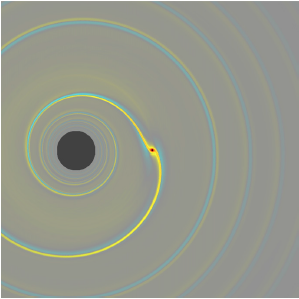
\includegraphics[scale=0.294]{figures/ch0/TypeI_Duffell}& \hspace{-0 pt}
%
 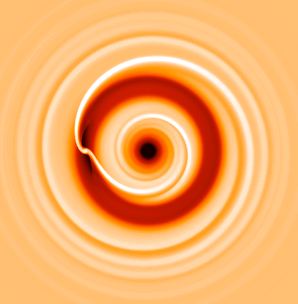
\includegraphics[scale=0.4]{figures/ch0/JupiterTypeII} &  \hspace{-0 pt}
%
 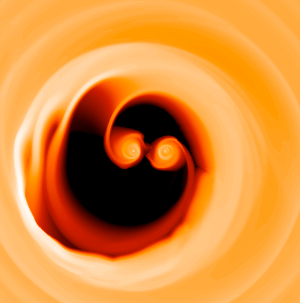
\includegraphics[scale=0.4]{figures/ch0/q1_CentralCav} 
\end{array}$
\end{center}
%\vspace{-0.35in}
%\caption{Snapshots of density from 2D hydrodynamical simulations for binaries on a fixed circular orbit, with increasing binary mass ratio from left to right ($q=10^{-6}, 10^{-3}, 1.0$). The Left panel is adopted from \citep{DM2012:gaps} and depicts the linear, Type I regime, the middle panel depicts teh Type II regime, and the right panel.} %
\caption{The left panel is for $q\equiv M_2/M_1 =10^{-6}$ (adapted from \citep{DM2012:gaps}), such a small secondary excites linear spiral density waves in the disk causing Type I inward migration of the binary. The middle panel is for a binary with $q=10^{-3}$, the dark ring in the orbit if the smaller BH is the low density gap leading to Type II migration. The right panel depicts the clearing of a central low density cavity around an equal mass binary.}
\label{Fig:IntroHydro}
\vspace{-0.2in}
\end{figure}
%%%%%%%%%%%%%%%%%%%%%%%%%%%%%%%%%%%%%%%%%%%%%%%%


\cite{LinPapa:1979a}, \cite{GT79}, and \cite{GT80} laid the groundwork for
disk interactions with very small mass ratio systems, where the response of
the binary and disk can be explored with linear perturbation analysis. In this
case, the secondary launches linear spiral density waves from the locations of
Linblad resonances in the disk \citep{LyndenBellKalnajs:1972}. Summing
contributions from torques exerted on the disk at these resonances,
\cite{GT80} were the first to show that the back-reaction of the disk
perturbations onto the binary cause the binary orbital separation to change.
For normal disk parameters (\emph{e.g.} outward decreasing disk density and
pressure), inward torques on the secondary from the outer Linblad resonances
outweigh the outward torques on the secondary from the inner Linblad
resonances, and inward `migration' (orbital shrinkage) occurs
\cite{Ward:1986}. This process, where linear spiral density waves are launched
by the secondary and cause the binary's orbit to shrink, is called Type I
migration \citep[See also][]{MeyerVernetSicardy:1987, Ward:1997, Tanaka:2002}.
Hence, the solutions to the equations of hydrodynamics, for disks perturbed by
a small mass ratio binary, consist of wave solutions launched form the
position of the secondary. In the frame of the binary, these waves have a
stationary phase and once they propagate into the disk on both sides of the
binary, the disk approaches a static solution which follows the secondary
component as it slowly changes its orbital radius and possibly eccentricity
(See Figure \ref{Fig:IntroHydro}) \citep{GT80, Ward:1988, GoldriechSari:2003}.





When the binary mass ratio is large enough, the spiral density waves launched
in the disk become non-linear at only a short distance (less than a disk scale
hieght) from the secondary \citep{GoodmanRafikov:2001}. The waves steepen into
a shock and deposit angular momentum to the disk material in the co- orbital
region of the secondary \citep{DongRafI:2011, DongRafII:2011, LinPapa, chapter3}. This
process clears a low density annulus in the orbit of the secondary.
\cite{LinPapa:1986b} were the first to point out that if such a gap is formed,
the secondary will be locked into the radial flow of the disc, migrating at
the viscous inflow rate. Such migration, when a gas barrier is formed around
the binary is called Type II migration \citep[see also][and Chapter 3]{Ward:1997, KleyNelson:2013, othertypeIIrefs}



Another important difference between different binary+disk systems is the
total gas resvoir. Analytical work by \citep{SyerClarke:95, Ivanov:1999}, in
one dimension,\footnote{averaging disk height and azimuth} showed that in the
non- planetary case, the Type II rate would eventually slow on scales where
the mass of the disc becomes smaller than the mass of the migrating binary
component. The argument being that there is no longer a large enough angular
momentum reservoir in the gas to shrink the binary separation on the viscous
timescale, hence, this `secondary dominated migration' would cause a pileup of
gas behind the secondary and the gas interior to the secondary's orbit would
drain onto the primary creating a central cavity devoid of gas and possibly
halting accretion onto the binary. Other 1D arguments \citep{other1Darguments} and even early 2D smoothed particle hydrodynamics (SPH)
simulations simulations \citep{Artymowicz:1991} concluded that the outward
torques from the binary would clear a cavity around most binary systems in the
Type II regime.


This picture, while laying the goundwork, has been greatly altered by work in
the intervening two decades, notably by the advent of two-dimensional
numerical, hydrodynamical simulations which capture the full non-axisymmetric
nature of the binary disk interaction, and allow global, time-dependent
solutions. The first of such numerical calculations was carried out in
\cite{AL94} and \cite{ArtyLubow:1996} who ran SPH simulations to
test analytic work that predicted the sizes of circumstellar disks in binaries
and the sizes of the central cavities surrounding the stellar binaries. These
SPH simulations showed that particles, in the form of streams tidally ripped
from the edge of the cavity wall, could indead flow past the binary tidal
barrier and reach the binary components. The ability of gas to flow past the
tidal barrier is of two-fold importance. First, it can allow high levels of
accretion onto the binary, which could generate a bright EM signature of the
binary, and second, it affects migration (and hence merger) rates of binaries
in gas disks \citep{DuffellFTV:2014}. The implications of both are currently areas
of active research. 




This picture, fails to account for mass flow across the gap along
horshoe orbits in the full dimentionlity of the problem. Recent work, using 2D
viscous hydrodynamical simulations has shown that mass flow accross the gap,
can allow the secondary to migrate at a rate depedent on disk parameters
(denisty, temperature, pressure), and limited by a maximum migraton velocity
which can be greater than the viscous rate \citep{Edgar:2008, DuffellFTV:2014,
DurmannKley:2015}. The mechanisms which dictate the migration rate of gap
openeing planets in the full two and three dimensional pictures is a topic of
ongoing work.


Additionally Chapter 3 of this thesis shows that the clearing of a central
cavity is not necessarily due to secular effects as in the picture of disc
dominated migration \cite{SyerClarke95}. Chapter 3 provides evidence that
the clearing of an annulus in the orbit of the secondary gives way to a much
more violent clearing of a \emph{central cavity} for mass ratios above $q
\sim0.04$.

Chapters 2 and 3 show also that the Type I to Type II regimes are not the only
that depend on mass ratio. For binary mass ratios above $q\sim0.04$, a mass
ratio well into the Type II regime for thin disks, the clearing of an annulus
in the orbit of the secondary gives way to a much more violent clearing of a
lopsided, \emph{central cavity} and time dependent bahavior. From mass ratios
$q \sim 0.3$ the lopsided central cavity is highlighted by an orbiting
overdensity at its inner wall. Chapters 2 and 3 provide more details on these
transitions and their importance for observing MBHBs.




The work in this thesis focuses on the implications for accretion onto the binary. Hence we now summarize the recent work on this front.


\cite{Haysaki:2007} conducted the first 3D-SPH simulations that specifically
targeted MBHB systems with the intent to measure accretion rates onto the
binary. \cite{Haysaki:2007} runs simulations of binaries with mass ratios
$q=1.0$ and $q=0.5$ and binary ecentricities $e=0.0$ and $e=0.5$ for up to 60
binary orbits. They find that streams are indeed pulled into a central, low
density caviy forming a triple disk system \citep{Hayasaki+2008} consisting of
the circumbinary disk and mini-disks around each binary component. The streams
promote accretion onto the BHs at rates as high as a tenth of the Eddington
rate. For eccentric binaries, \cite{Haysaki:2007} found a strong modulation in
the accretion rate at the binary orbital period. 
%Cons - run for a short time at low resolution, injection of particles at r=1.65 seems artificial

The SPH simulations of Hayasaki were soon succeeded by the 2D, grid based,
adaptive mesh refinment simulations of \citep[][hereafter MM08]{MacFadyen:2008},
 run for 1000's of binary orbits (greater than a viscous
time at the position of the binary). These higher resolution simulations,
using the FLASH code \citep{Fryxell:2000}, are more adept at capturing
supersonic dynamics in the vicinity of the binary (shocks). Though
MM08 cut out the inner region of the domain containing the
binary, they measure accretion rates into the inner boundary which is inside
the low density (besides the streams) central cavity set by the initial
conditions. The high resolution simulation of MM08, for an
equal mass binary, found new behavior: the elongation of the central cavity
which results in high levels of accretion into the inner simulation boundary.
The resulting periodogram of the accreation rate  has the strongest peeks at a
low frequency peak near $4.5 \times$ the binary orbital period and at twice
the binary orbital period. They not discussed in MM08, the cause of accretion
variabiltiy at these timescales is elucidated in Chapter 2 of this thesis and
also \citep{ShiKrolik:2012} below.


Further SPH studies of MBHB systems were conducted by \citep{Cuadra:2009} who
3D simulations at a resolution $10 \rightarrow 100$ times higher than that of
\cite{Haysaki:2007} for marginally self-gravitating discs with a binary mass
ratio of $q=0.3$ and a simple cooling prescription for the gas. They do not
find elongation of the cavity as in MM08, though this could be due to the
short amount of time for which the simulations are run, $\sim 200$ orbits, or
the resolution loss that SPH simulations suffer in low density regions (namely
the dynamically import cavity edge of the circumbiary disk).
\citep{Cuadra:2009} do find an accretion rate variable at the orbital period
and a propensity for the gas disk to excite binary eccentricity.
\citep{Cuadra:2009} also finds that the smaller has a larger ($\times 2$)
accretion rate than the secondary due to its closer proximity to the edge of
the central cavity.


\citep{Roedig:2011:trqs} carry out similar simulation to \citep{Cuadra:2009}, except they start the binary at different initial eccentricities $e_0$ finding that eccentricity damps for $e_0 \gsim 0.6$ but is excited for $e_0 \lsim 0.6$, suggesting the existence of rather large a preferred binary eccentricity. \citep{Roedig2012:eccevo} consider different disk thermoydnamics and different accretion (sink) perscriptons. In both cases the accretion rates onto these eccentric binaries  found to have periodicity at the binary period and its harmonics, but also at lower frequency disk periods and beat frequencies between disk and binary periods.


The first magneto-hydrodynamical (MHD) simulations of the circumbinary disk
were carried out by \cite{ShiKrolik:2012} with a grid based code.
\cite{ShiKrolik:2012}  perfomed both 2D hydrodynamical and 3D MHD simulations
of an equal mass binary on a circular orbit with a similar setup to
\citep{MacFadyen:2008}. Despite a higher overall accretion rate due to larger
viscous stresses generated by the Magneto-rotational instability (MRI),
\cite{ShiKrolik:2012} find similar results to MM08, in that they also find the
growth of a lopsided central cavity (elongated with a cavity wall
overdensity), which generates variable accretion into the central simulation
domain. The variablity of the accretion rate is in agreement with MM08,
exhibiting a long period variation at the period of gas orbits int the cavity
wall and a second period at twice the binary orbital period (due to the
symmetry of an equal mass binary). \cite{ShiKrolik:2012} provide evidence that
the cavity lopsideness is due to the kinematics of stream impacts and
recycling of the cavity wall overdensity: the cavity wall overdenisty
periodically shears apart, causing a lump to orbit around the cavity, feeding
streams which are flung out of the cavity again to generate the cavity wall
overdensity. \cite{ShiKrolik:2015} have extend upon the above work by
considereing a range of binary mass ratios, finding qualititve agreement with
\cite{DHM:2013:MNRAS} and \cite{Farris:2014} discussed below.

MHD simulations by \citep{Noble+2012} incorporate post-Newtonian corrections
to the disk hydrodynamics and binary orbital decay in order to track the disc
response through binary inspiral. \citep{Noble+2012} find that gas can follow
the binary down to separatios of $\sim10M$ with $10 \rightarrow 20\%$
reduction in accreation rate. They also find a lopsided central curcumbinary
disk cavity, in agreement with MM08, \citep{ShiKrolik:2012}, and the works
that we discuss next.

Chapter 2 of this work \citep{DHM:2013:MNRAS}, extends the work of MM08 (using
the same numericla code and a similar numerical setup) by considering not only
equal mass binaries but range a mass ratios from $q=0.01 \rightarrow 1$. The
qulatative results of disk response and accretion rate variability found in
MM08 and \citep{ShiKrolik:2012} are reproduced and compared to the magnitude
of accretion for a point mass. By varying $q$, however, a landscape of
accretion variabiltiy and mangitude is uncovered and discussion of its use for
MBHB searches is discussed.

\citep{Farris:2014} extended the work of \citep{DHM:2013:MNRAS} by adapting the
moving mesh code DISCO \citep{Duffell:2011:TESS,
DuffellMHDDISCO:2016} to track, for the first time, gas dynamics in the
vicinity of the binary components using a grid based (rather than an SPH)
code. \citep{Farris:2014} finds results in agreement with MM08 and
\citep{DHM:2013:MNRAS} and finds also that the relative accretion rate onto
each black hole is a function of mass ratio, dominated by the secondary from
$0.05 \leq q < 1$. 


For the equal mass case \citep{Farris:2015:GW} considered
the effects of gravitaional wave decay on the CBD system showing that gas
could indeed follow the binary to small separations causing variable accretion
up until merger, contrary to previous lore that gas should be left behind in a
`decoupling phase' by a binary that is quickly merging due to GW emission.
Finally \citep{Farris:2015:Cool} implemented a simple cooling prescription in
DISCO (previous work being for isothermal disks) showing that the variability
of the accretion luminosity should indeed follow what was predicted in
previous works for the variabiltiy of the accretion rate.



Recent work has examined the nature of gas temperature on accretion rates,
both \cite{YoungClarke:2015} and \cite{RagusaLodato:2016} use SPH codes (2D
and 3D repectivley) to simulate a range of binary mass ratios above $q=0.1$
and vary the gas temperature. In these simulations, the gas temperature
manifests in the form of the disk vertical height to radius aspect ratio,
$h/r$ which, in vertical hydrostatic equilibrium, is equal to the ratio of the
sound speed to the gas angular orbital frequency at distance $r$ from the
system barycenter. A thicker disk, is hotter and has larger pressure forces.
Both studies find that, while simulations in the literature (using $h/r \sim
0.1$) accrete at near the value for a single BH, more realistic, colder AGN
discs ($h/r \sim 0.01$) should accrete at much lower rates. Though
interesting, the robustness of these results remains to be seen as numerical
difficuties arise in cold disks, especically when using SPH codes \citep{}.


Notably, \citep{RagusaLodato:2016} simulations capture the lopsided disk
behavior with a circular binary. Except for a study which considered an
eccentric binary \citep{Dunhill+2015}, no SPH simulations have captured the
lopsided disk behavior. It is not yet clear however what has allowed this
change. The SPH works to date are computed with different numerical codes, at
different resolutions, and for different total numbers of binary orbits.


In addition to prograde disks in the plane of the binary, some groups have alse considered retrograde disks \citep{Nixon+2011, ReodigSesana:2014, BankertShiKrolik:2015, AmaroSeoane:RetroDiscs:2016} and the alignemnt or tearing of warped disks \citep{Nixon+2012, Hayasaki+2013, Nixon+2013, DoganNixonKingPrice:2015}.

As a final note in this review of numerical simulations of CBDs, full MHD
simulations in general relativity (GRMHD) have been carried out by
\cite{FarrisLiuShap:2010:Bondi, FarrisShap:2011, FarrisGold:2012,
Gold:GRMHD_CBD:2014, Gold:GRMHD_CBDII:2014} in the regime just before merger,
showing also that accretion rates can be of order the rate expected onto a
single BH, periodic, and the gas can follow the binary down to separations of
order a few $M$, allowing the binary to be bright up until merger.


% Stil need to add:
% Noble
% MunozLai:2016 - ecc stars accretion rates




%%%Observations
\subsection{Observations of MBHBs}

%%%%%%%%%%%%%%%%%%%%%%%%%%%%%%%%%%
%%%FIGURE doppler candidates
%%%%%%%%%%%%%%%%%%%%%%%%%%%%%%%%%%
\begin{wrapfigure}{R}{0.5\textwidth}
%\begin{figure}
\begin{center}
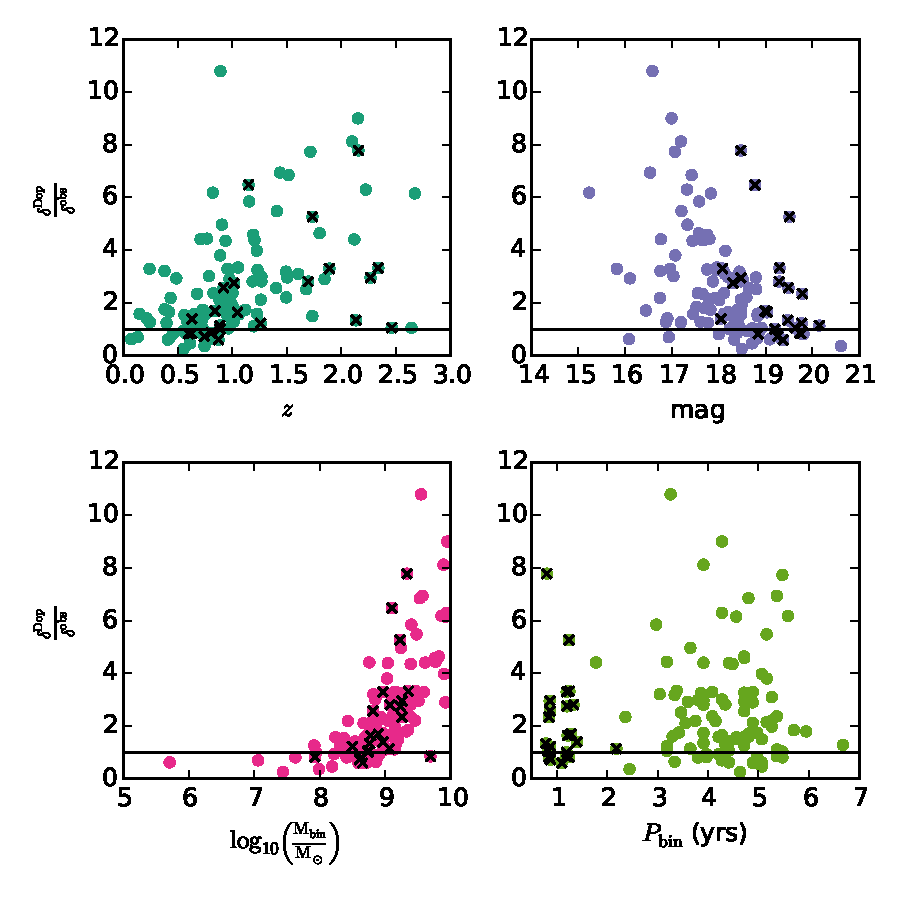
\includegraphics[scale=0.55]{figures/ch0/PTF_xsiGtr1_vs_z_M_P_alph_I90} 
\end{center}
\caption{A subest of the MBHB candidates from \citep{Graham+2015b} and \citep[][denoted by black x's]{Charisi+2016} for which spectral slopes are measured and the magnitude of variabiltiy form Doppler boosting can be estimated. From left to right, top to bottom, the ratio of predicted Doppler variability amplitude to observed variability amplitude is plotted vs, redshit, average optical magnitude, log mass, and observed period. Candidates above the horizontal black line are possible Doppler beaming MBHB candidates.}
\label{Fig:Contour}
%\end{figure}
\end{wrapfigure}
%%%%%%%%%%%%%%%%%%%%%%%%%%%%%%%%%%%%%%%%%%%%%%%%


As discussed, a motivation for the above theoretical calculations is to
determine the types of EM signatures that will identify MBHBs in the inspiral
regime. Searching for MBHB by searching for periodically varying AGN has been
proposed before by MM08, \cite{Haiman+2009}, and by HKM09.
 

HKM09 propose that close MBHBs can be indentified in Quasars by their production of EM emission moduated at the binary orbital period. Under this assumption they compute the duty cycle of MBHBs with periods observable in human lifetimes by computing the residence times of MBHBs at a given orbital period (binary separation) taking into account gas induced migration and also GW driven inspiral. Comparison of the residenc etime to the averge Quasar liftime allows HKM09 to predict the size of an EM time domain survey required to capture a specified number of MBHBs at agiven orbital period and luminosity.

%caluclate the duty cycle of MBHBs with 

%assume that MBHB can generate periodic EM signatues at the binary orbital period to predict the sample size of Quasars needed to detect a sample of MBHBs that should be needed based on Quasar lifetimes and gas + GW induced binary shrinkage. 




These predictions came to fruition only a year ago when the a group from
Caltech/JPL scoured 9 years of time domain optical photomoetry of
$\sim250,000$ quasars in the Catalina Real Time Transient Survey
\citep{CRTS1:Drake:2009, CRTS2:Djorgovski:2010, CRTS3:2011Mahabal,
CRTS4:Djorgovski:2011} attempting to characterize quasar variability. They
found a subset of periodically varying sources. The brightest of these sources
is PG 1302-102 which was identified as a close, $a \sim 0.01$pc separation
MBHB candidate, the first identified in this manner, and the closest reported
binary separation at the time \citep{Graham+2015a}. The second part of Part I
of this thesis uses the theoratical developments of the first half to
interpret the binary candidate PG 1302, finding that PG 1302 is most likely
described by a system with a disparate mass ratio where the smaller BH is
emitting most of the optical light and modulating it via relativistic Doppler
boosting.


Soon after the announcement of PG 1302, 110 more MBHB candidates, were picked
out of the CRTS for their periodic optical light curves \citep{Graham+2015b}
and then 33 more, at shorter periods \citep{Charisi+2016}, from the
Palomar Transient Factory (PTF) \citep{PTF}. In addition to these mass candidae
discoveries, a few single candidates were also announced from time domain periodicity arguments: A proported 


Follow up observations are needed to secure the nature of these candidates. As
Jules Halpern says: `periodicity is the easiest thing to prove in astronomy,
you just have to wait'. However, furhter evidence, across the
wavelengths can help pin down the mechanism driving such peridocity and work
must be done to place these MBHB in their full environment of gasy, dusty
active galactic nuclei. A full multiwavlength picutre of the variable MBHB
candidates must be peiced together. The final chapter of Part I (Chapter 5) is
a beginning to this process, presenting a model for the infrared variability
expected from dust reverberation by MBHBs that exhibit variable emission,
through either accretion variablitiy or anisotropic Doppler boosted emission.









% I want to note here 
% (0) intrinsic quasar variability
% (1) that the above searches might exclude binaries with multiple freqeuncies due to naure of wavelet analysis
% (2) Calculation of whether these 144 coudl be Doppler beamed plus figure.
% (3) MBHBs candidates claimed since with plusses or minuses
%  the search continues: \citep{Tamara:2015}
% 	spectroscopic methods:
% 	 BLRs:
% 		\citep{DecarliDott:2013:SpecMBHBcandI}
% 		 Halpern's group?
%      CBD cutoffs:

%      EM time domain
%       Graham a, b
%       Charisi+
%       Zheng, Z.

% (4) IR STUFF JUN ET AL AND CHAPTER 5!



%picture has been altered in the last decade...



% The advent of numerical simulations which capture the 2D, non-axisymmetric
% nature of the binary disk interaction also found that accretion onto the
% binary is not halted by a the torque barrier of the binary, rather accretion
% rates can even be increased from the point mass steady accretion case because
% teh binary can vioently pull streams of gass form a circumbinary cavity edge.
% The gas from these streams forms mini-disks around each binary component....
% explain accretion process with figure with vectors...

%Chapter 2 provides evidence for further birfurcations
%for near equal mass ratio systems and Chapter 3 elaborates on the physical
%mechanisms driving the more subtle of these transistion.








% %%% 1D Summary
% Early papers: 
% 	Type I: 
% 		Lynden-Bell and Kalnajs 1972 - resodnances and spiral arms in galactic setting
% 		Lin and Papaloizou 1979 a - angular momentum transport:Type I migration - tidal truncation of CBDs - application to dwarf novae
% 		GT 1980 - first to suggest migration - from resonant tides
% 		Meyer Sicardy - 


% 	Type II
% 		Syer Clarke Disk vs sec dominated - app to MBHBs
		
% 		b - Tidal truncation of CBDs applied to contact binaries and the formation of commensurable satellites in the solar system.
% 		Lin and Papaloizou 1986 a - full nonlinear interaction f disk and sattelite, self grav, range of c_s and nu - density wave propagation studied- applied to protoplanet and the primordial solar nebula
% 		b - dynamical evolution of the disk and the orbital migration of the protoplanet in a self-consistent manner is considered - Type II viscous evolution rate derived here - numerical stuff?
% 		Lin Papa 1993

% 	Gap Clearing 
% 		The above Lin Papa papers
% 		Arty and Lubow 1994, 1996
	
% 	Both:
% 	Hourigan Ward 1984
% 	Ward 1997

% 	Eccentricity excitation/damping
% 	Ward 1988
% 	Goldreich Sari 2003

% Present day answers to earlier work:
% Type I:
% Rafikov and Dong etc
% Duffell

% Type II:
% Edgar 2008
% FTV Duffell 2014
% Durman and Kley? 2015

%Syer and Clarke: secondary BH can clear a gap in the CBD, and bank up material behind it, causing a change in the spectarl and possibly continuum emission from the AGN. They also introduced the idea od Type II secondary dominated vs. disk dominated mogration.

% Retrograde and warps alignment
% Nixon+2011 - retro
% Nixon+2012 - alignment to retro of misaligned
% Hayasaki+2013 - warped/alignment
% Nixon+2013 - tearing up the disc - misaligned
% ReodigSesana:2014 - retro vs pro
% DoganNixonKingPrice:2015 - tearing up misaligned
% BankertShiKrolik:2015 - retro
% Amaro-Seoane+2016 - retro

% EMPHASIZE THE QUESTIONS IN THIS THESIS: Can accretion make EM signature of MBHB and can we use it to identify a pop of MBHB candidates?





































\section{Part II: Stellar Black Hole + Neutron Star Binaries}
%EMPHASIZE THE QUESTIONS IN THIS THESIS: What is the BH battery EM signature of non-disrupting NSBH binaries?
%

The merger of NSs and stellar BHs will generate GWs detectable by the Laser
Interferometer Gravitational-Wave Observatory \citep[LIGO][]{aLIGO:2015}.
Binaries with BHs will generate the highest amplitude GW signals \emph{e.g.}
Eq. \ref{Eq:BinStrain}, but a binary containing a NS has the most potential to
produce a bright EM signal, making BHNS systems especially interesting sources
of EM+GW emission.


%%%%%%%%%%%%%%%%%%%%%%%%%%%%%%%%%%
%%%FIGURE BHNS TDs
%%%%%%%%%%%%%%%%%%%%%%%%%%%%%%%%%%
\begin{wrapfigure}{R}{0.4\textwidth}
%\begin{figure}
\begin{center}
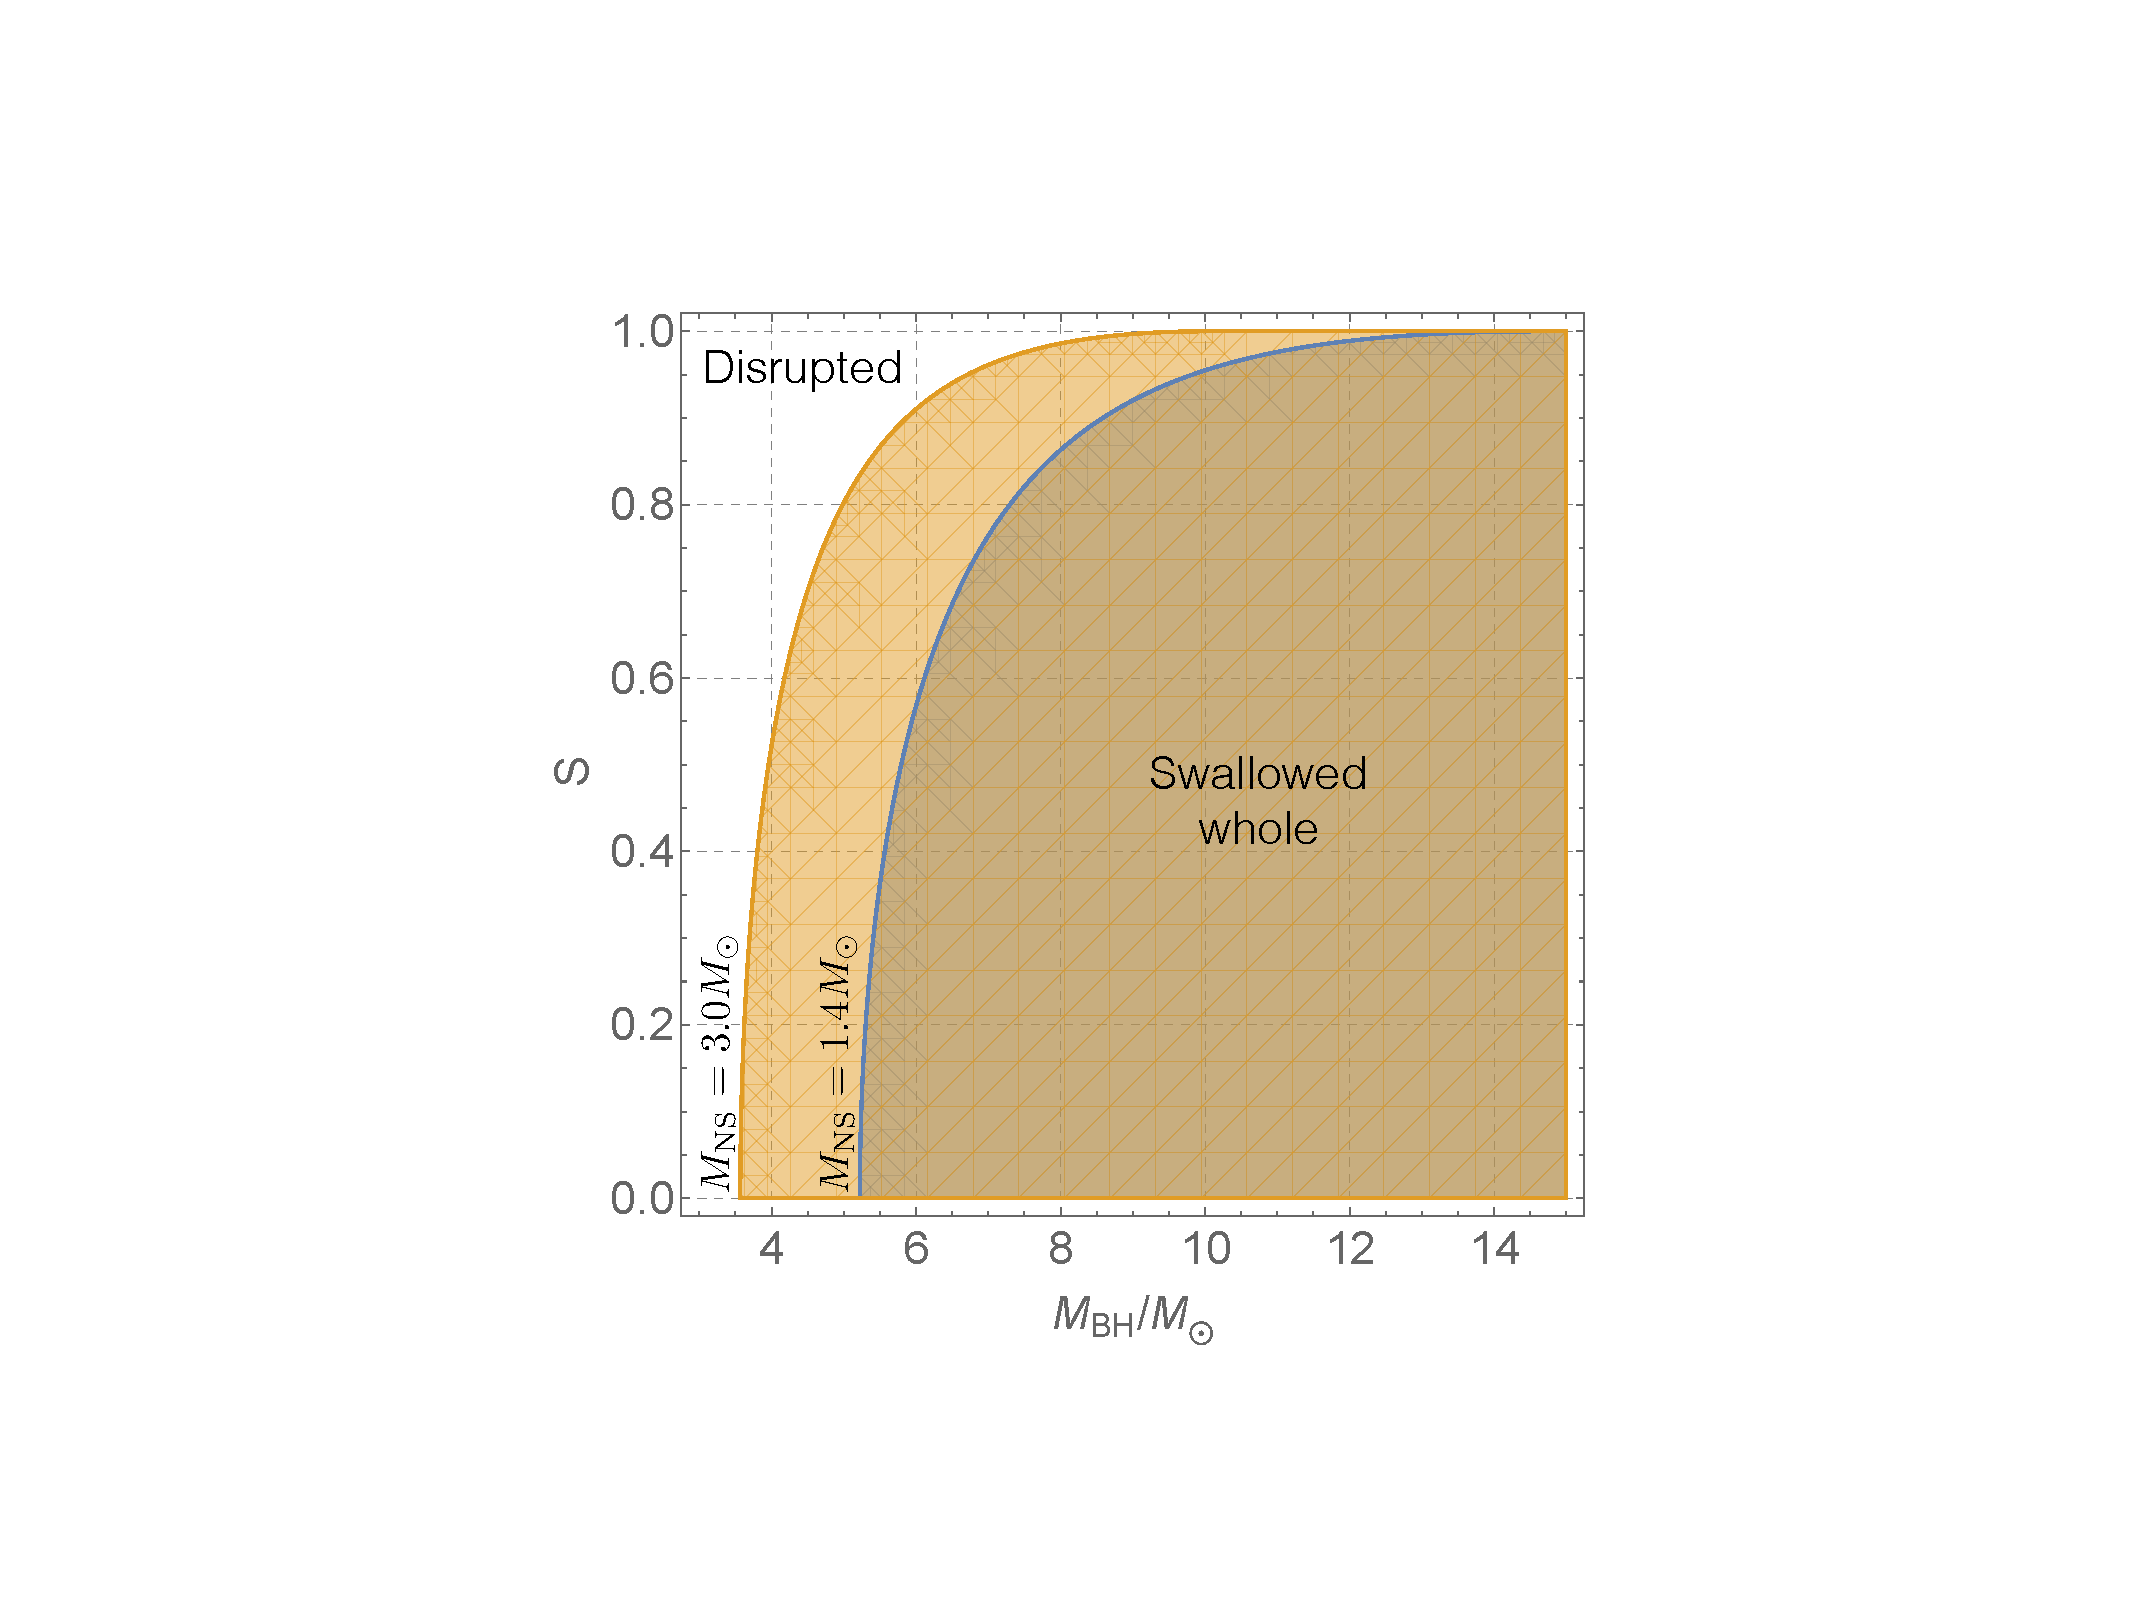
\includegraphics[scale=0.33]{figures/ch0/BHNS_TDs} 
\end{center}
\caption{Approximate values of black hole mass and spin for which a companion neutron star would be disrupted outside of the black hole horizon. Each of the two regions are for the labeled neutron star masses spanning the range of theoretical limits and for a neutron star with radius of 10km.}
\label{Fig:Contour}
%\end{figure}
\end{wrapfigure}
%%%%%%%%%%%%%%%%%%%%%%%%%%%%%%%%%%%%%%%%%%%%%%%%

The tidal disruption of a NS by its BH partner could generate a $\gamma$-ray
burst after merger \citep{NPP:NSBH_GRB:1992}. However, it is under-appreciated
that most BHs should be large enough to swallow their NSs
whole, causing the mergers of most BHNS binaries to be dark. Figure 
\ref{Fig:NSBH_TDs} plots the simplest approximation for the disruption,
\begin{equation}
 r_T \approx \left( \frac{M_{\rm{BH}} }{ M_{\rm{NS}}} \right)^{1/3} R_{\rm{NS}} \geq r_H(S) 
 = M_{\rm{BH}} + \sqrt{M^2_{\rm{BH}} + S^2},
\end{equation}
which requires that the disruption radius be outside of the BH event horizon
with dimensionsless spin $S$ (using natural units for the black hole horizon
radius). \ref{Fig:NSBH_TDs} shows that, unless the BH has near maximal spin,
BHNS systems with $M_{\rm{BH}} \gsim 6 \msun$ will swallow the NS whole! This
is of course a crude aproximation which depends on the (unknown) equation of
state of the NS. More sophistaced approximations, however, do not find anything
drastically different \citep[\emph{e.g.}][]{Foucart:2012}.


Although the distribution of BH masses which will merge with
a NS is unknown, it is interesting to note that the BH mass distribution
inferred from BHs in X-ray binaries peaks around $8 \Msun$ \citep{Ozel:2010}
and the only known BH binary consisted of BHs with masses $\sim 30 \Msun$, which
would certainly swallow a NS hole. Though suggestive, it is important to keep
in mind that each of these formation channels may be independent, and not
applicable to a BHNS system.

As additional motivation, LIGO is the most sensitive at a frequency of $\sim
200$ Hz, this is the gravitational wave frequency at coalescence for a NS of
mass $1.4 M_{\Msun}$ in a circular orbit with a BH of mass few $\sim100
\Msun$. If such binaries occur in nature, they have the potential to be high
signal to noise LIGO detections, and will certainly not disrupt the NS. The
above motivates an exploration of EM counterparts to non-disrupting NSBH
systems.


A possible pathway for bright EM emission by non-disrupting BHNS mergers is
through the electromegnatic interaction of the NS magnetosphere and the BH
event horizon. 

Paragraph about all the diff astro mechanisms for UIs.
% The NSBH system behaves analogously to a unipolar inductor, which has been investigated in application 
% to a number of other astrophysical systems, \textit{e.g.} Jupiter and 
% its moon Io \citep{GLB:1969}, planets around white dwarfs \citep{Li:1998} and main sequence stars \citep{LaineLinI:2012,LaineLinII:2012}, 
% binary neutron stars \citep{Vietri:1996,Piro:2012, DLai:2012, Palenzuela:2013}, 
% compact white dwarf binaries \citep{Wu:2002, Dall'Osso:2006, Dall'Osso:2007, 
% DLai:2012}, BHs boosted through magnetic fields 
% \citep{Lyut:2011, Penna:2015}, and the Blandford-Znajek (BZ) mechanism \citep{BZ:1977} for a single BH spinning in a magnetic field  \citep[for recent numerical work on the BZ mechanism see \textit{e.g.}][]{PalenzuelaBZ:2011, Kiuchi:2015}. The calculation for NSBH systems, 
% already presented in Ref.\ \cite{McL:2011}
% and confirmed in the detailed relativistic analysis of
% Ref.\ \cite{DorazioLevin:2013}, as well as the numerical calculations
% of Ref.\ \cite{Paschalidis:2013}, gives the scaling of power available
% for conversion into electromagnetic luminosity. In the next section we
% will consider the implications of throwing this power into luminous
% elements in the BHNS circuit.

To introduce this mechanism, I want to first introduce a
similar, though subtle example of the Faraday-Disk. The Faraday disk is a type
of unipolar inductor constructed by placing a conducting rod through the
center of a conducting disk, and running a wire from the top of the rod to the
outer edge of the disk, where a sliding contact completes a circuit (see
Figure \ref{Fig:FDschem}). Tracing a magnetic field perpendicularly through the disc, and
spinning the disk generates a elecromotive force, $\xi$. We can compute the
voltage drop from the center of the disk, to the edge of the disk, from
Faraday's law 
\begin{align} 
\xi = - \frac{1}{c}\frac{d}{dt}\int_{\Sigma(t)}{\Bvec \cdot d\Avec} 
\end{align} 
where the circuit bounds an open, time-dependent surface $\Sigma(t)$. At first
glance, it seems that the emf should be zero, as the obvious loop (loop $a$ in
Figure \ref{Fig:FDschem}) connecting wire to disk to rod has zero magnetic
flux. However, Faraday disks do generate an emf, and this is easily verified
by considering the Lorentz force on electrons. To see this from Faraday's law, recall two restrictions in our
choice of the open surface of integration $\Sigma(t)$: 1) $\Sigma(t)$ must be bounded by the closed loop through which the emf is computed, and 2) $\Sigma(t)$ must capture the relative motion of the circuit.
%\begin{enumerate} 
%\item $\Sigma(t)$ must be bounded by the closed loop through which the emf is
%computed. 
%\item $\Sigma(t)$ must capture the relative motion of the circuit.
%\end{enumerate}
The key is in the second point: the part of the circuit that starts in the
disk must move along with the spinning disk, otherwise you implicitly assume
that the sliding contact and the disk are not in relative motion - but they
are by construction.


%%%%%%%%%%%%%%%%%%%%%%%%%%%%%%%%%%
%%%FIGURE Faraday Disk
%%%%%%%%%%%%%%%%%%%%%%%%%%%%%%%%%%
\begin{wrapfigure}{R}{0.4\textwidth}
%\begin{figure}
\begin{center}
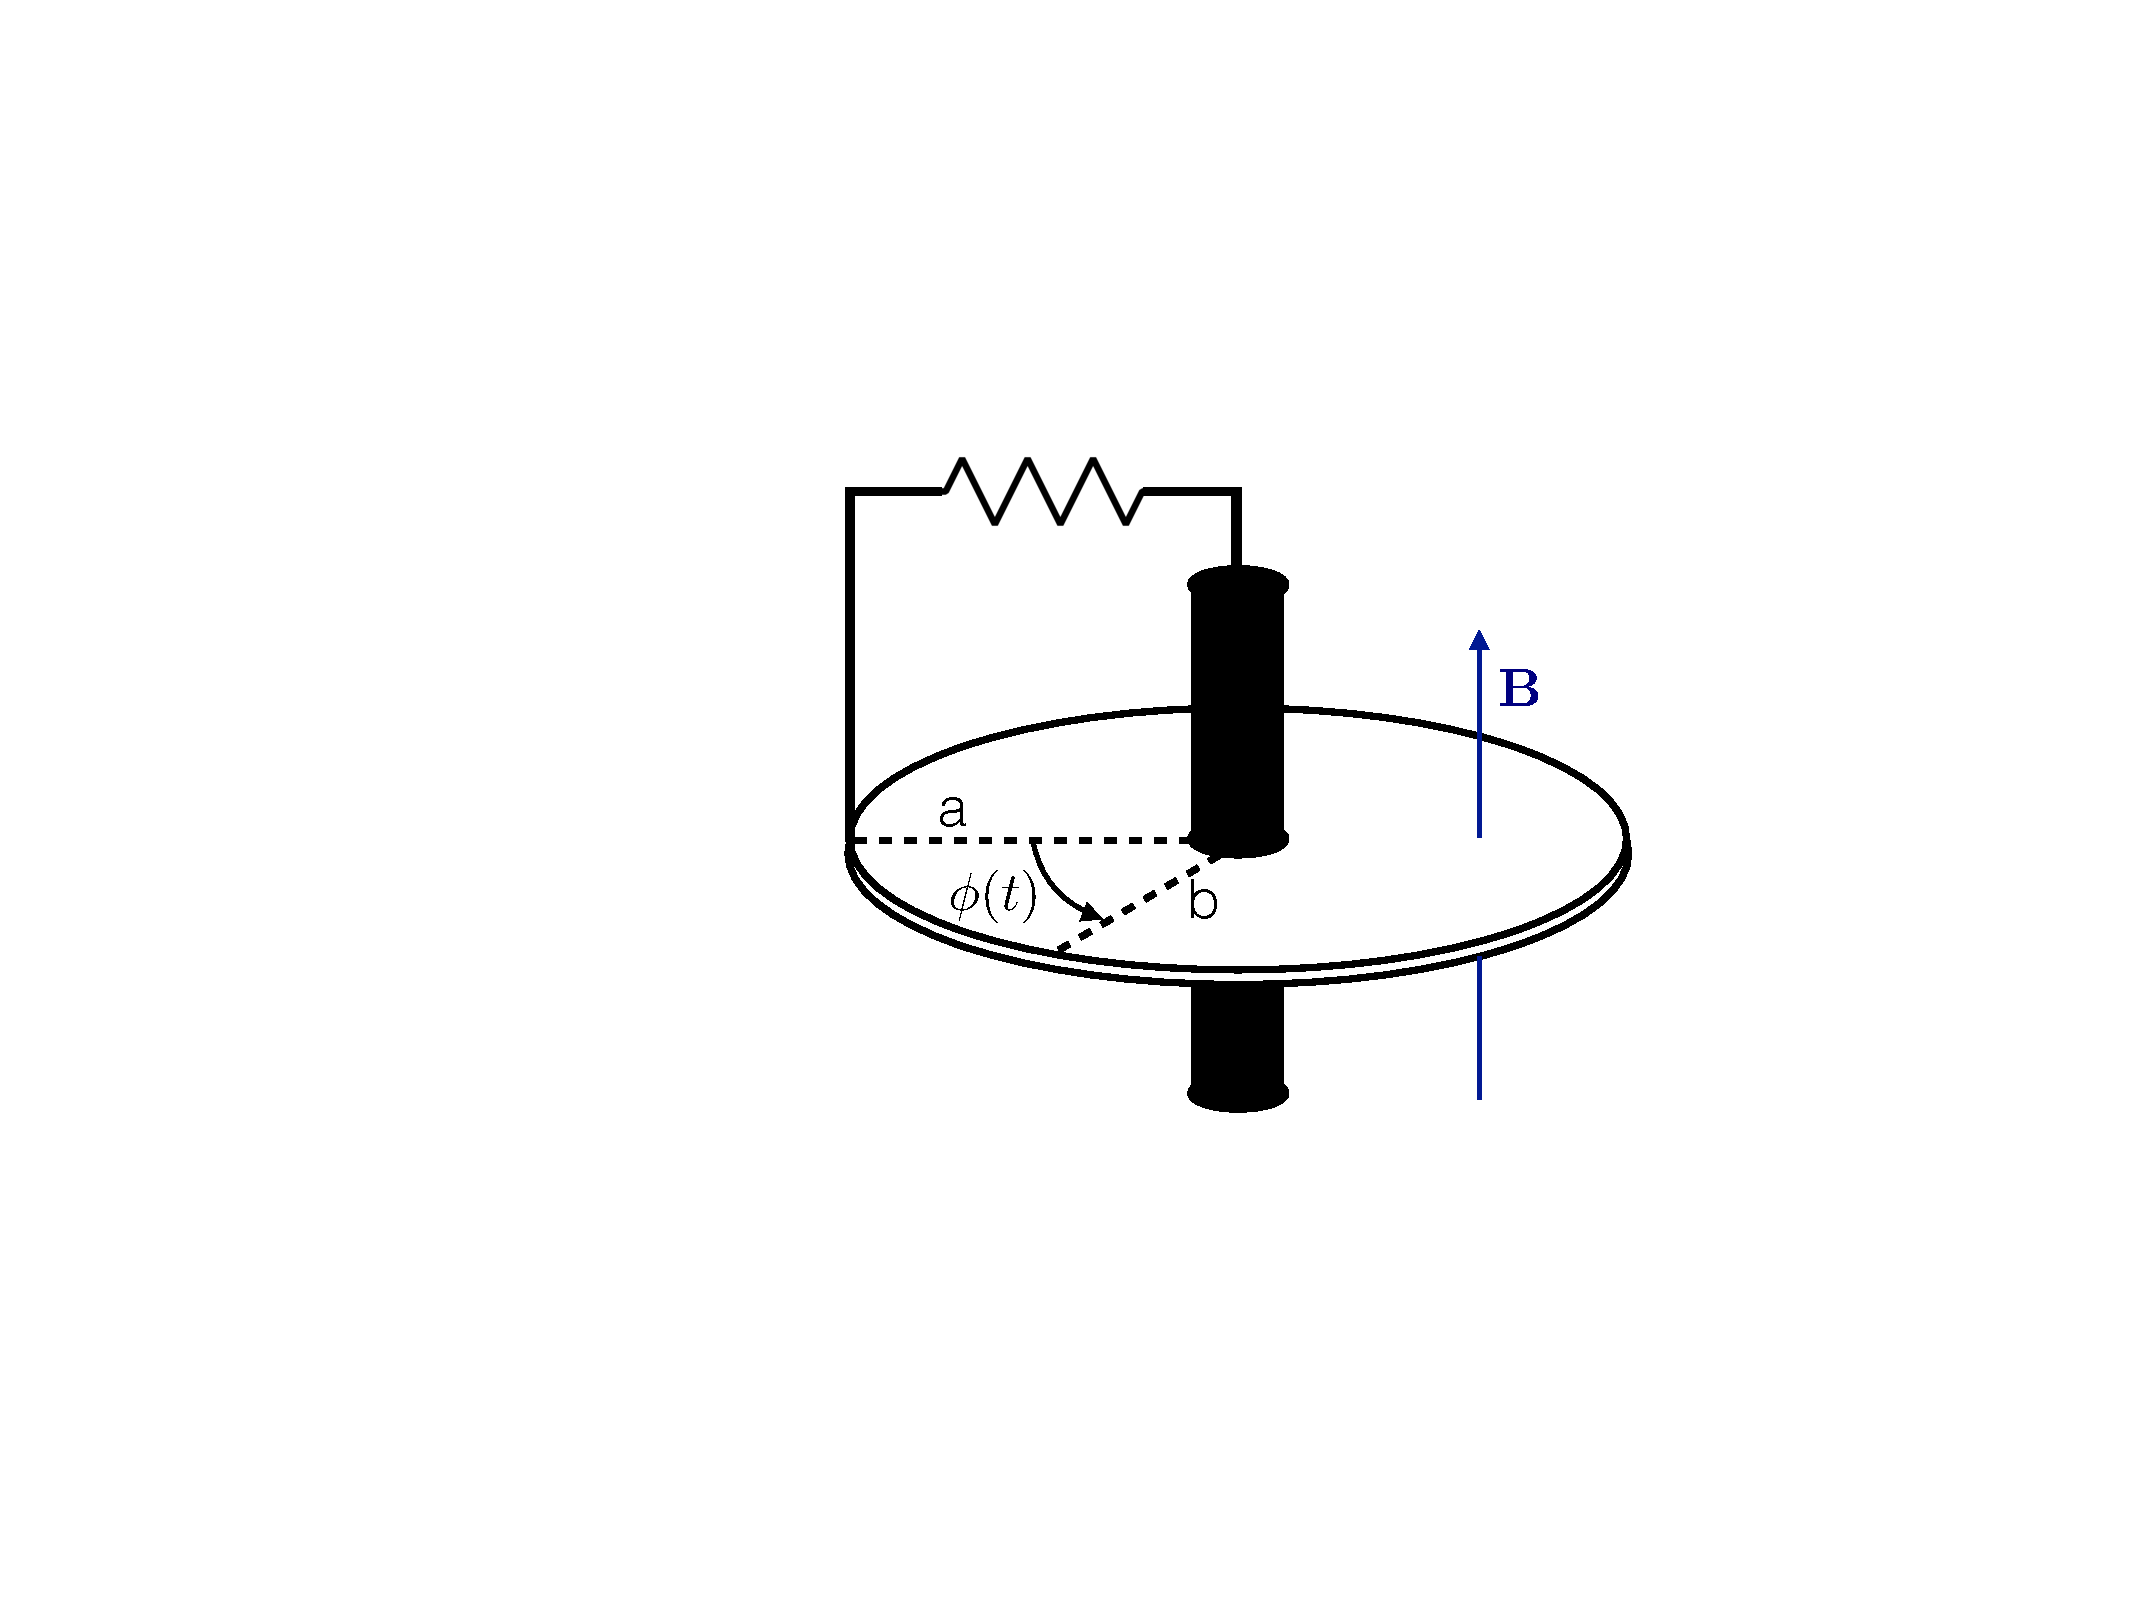
\includegraphics[scale=0.33]{figures/ch0/UI_schematic} 
\end{center}
\caption{Schematic of a Faraday Disk (unipolar inductor).}
\label{Fig:Contour}
%\end{figure}
\end{wrapfigure}
%%%%%%%%%%%%%%%%%%%%%%%%%%%%%%%%%%%%%%%%%%%%%%%%


To calculate the emf, choose loop $b$ in Figure \ref{Fig:FDschem} which moves
along at the rate of the spinning disk, $\Omega = d\phi/dt$. Say that the
radius of the disk is $R$ and the uniform magnetic field tracing the disk is $B$, then, working in polar coordinates $(r, \phi)$,
\begin{align}
\xi_{\rm FD} &= - \frac{1}{c} \frac{d}{dt} \int_{\Sigma(t)}{\Bvec \cdot d\Avec} =  - \frac{1}{c} \int^{\phi(t)}_{0} \int^{R}_{0}{B r dr d\phi}  \\
&= - \frac{1}{c} \int^{\phi(t)}_{0}{\frac{1}{2}\frac{\partial B R^2}{\partial t} d\phi} -  \frac{1}{c} \frac{B R^2}{2} \frac{d\phi}{dt}  = -\frac{B R^2}{2c} \Omega
\end{align}
where we have used Liebniz's rule of for integration with a time changing limt of integration. 

Remarkably, it turns out that the Faraday disk behaves similarly to a BH
moving through a magnetic field. The analogy is spelled out in \S \ref{}, but
if we take for now that the BH orbitting the NS acts as a conductor with size
equal to its event horizon \citep{MPBook}, then we can calculate the emf
generated by the NSBH system. 

All of the above reasoning holds for the BH battery, but instead of sliding
wires, we have moving B-feild lines which both act as wires (because electrons
are bound to them) and also generate the magnetic flux through the moving BH
horizon. Take our circuit in the BH-battery case to be the B-field gong form NS surface to a time dependent boundary on the BH horizon. Take the B field to be
that of a dipole attached to the NS, $B = B_{\rm NS} R^3_{\rm NS} r^{-3}$ and
consider two field lines separated by distance $R_H$ and moving in the $x$
direction relative to the horizon at speed $v_f$. then we find an result for
the horizon voltage analogous to the Faraday Disk case, and nearly identical
to that derived in \S \ref{7.1.1},
\begin{align}
\xi_{\rm BH} &= - \frac{1}{c}\frac{d}{dt} \int_{\Sigma(t)}{\Bvec \cdot d\Avec} =  - \frac{\pi R_H}{c} \int^{v_f t}_{0} {B(r) dx}  \\
&=  - \frac{\pi R_H}{c}  \int^{v_f t}_{0}{ \frac{\partial B(a)}{\partial t} dx}  - \pi R_H B(r) \frac{v_f}{c}    \\
& \sim    -R_H \left[r \frac{\left(\Omega_{\rm bin}  - \Omega_{\rm NS}\right)}{c} + \frac{R_H\Omega_{BH}}{c}\right] B_{\rm NS}  \left( \frac{R_{\rm NS}}{r} \right)^3
\end{align}
which is the maximum voltage over one hemisphere. There an infinite number of these circuits at all times. 

In the case of the Faraday Disk, the energy which can be harvested
electromagnetically, \emph{e.g.}, by heating the resistor in Figure
\ref{Fig:FDschem} to light a bulb), comes from the energy put into spinning
the disk. In the case of a BHNS binary, the electromagnetic potential energy
of the induced horizon voltage comes from the binary orbital energy, and as
detailed in Part II of this thesis, the available electromagnetic energy could
power luminosities observable from galactic distance (kpc) out to comsic
distance (Mpc) depending on the NS magnetic field strength at merger.


This result, that NSBH binaries could power high luminosity EM counterparts
without disrupting the NS was first put forth by
\cite[ML11][]{McL:2011}. This work was then expanded upon by
Chapter 7 of this thesis \cite[DL13][]{DL:2013:PhRvD}, which finds relativistic
solutions for the dynamics of a magnetic dipole, in arbitrary motion outside
of a horizon. 

Numerical works have recently tackled this problem in general relativistic,
force-free simulations, which solve the Einstein-Maxwell equations in the
limit that $\Evec \dot \Bvec$ is everywhere zero, and hence there are no
accelerating forces on electrons \citep{Paschalidis:2013}. Both types of
simulations estimate the observable luminosity via a Poynting flux measured at
the outer edge of the simulation domain. The simulation estimates match the
analytic arguments of ML11 and DL13. However, a true understanding of the
emission from NSBH systems requires more than this; it requires a radiation
maechanism, somethign to stick into the BH-batterey circuit that will shine.

The emission of EM radiation ultimately must come from dissipation of the BH-
battery power in the joint BHNS magnetosphere. The classic paper by
\cite{GJ:1969} shows that if a spinning NS, immersed in its own magnetic dipole
field, generates an electric field with components perpendicular to the
magnetic field, then electrons will be ripped from the NS crust. The
acclerating electrons emit curvature radiaiton which interacts with the
electromagnetic field to generate pair electron-positrons pairs which go on to
genreate more curvature radiation and a pari cascade ensues. The pairs move to
screen accelerating electric field (components of $\Evec$ parallel to
$\Bvec$), until a force-free condition is met, and the NS is surrounded by the
magnetosphere of \citep{GJ:1969}. Such a situation halts dissipation of the BH-battery power. 

However, this does not stop pulsars from shining.  As \citep{RudSuth:1975} pointed out, the force free condition cannot always be sustained globally in the NS magnetosphere, for example, (). In these gaps, particles are still acceleratd and dissipation allows the release of EM radiation.

We assume that a similar situation is at play in the NSBH example. There need only be gaps in the forece free magnetosphere, or magnetic reconnetion (though I am not sure how this would occurr) to release the BH battery power. In Chapter 8, we envision such a mechansim, which results in a fireball soon after merger emitting in the hard x-rays and soft $\gamma$-rays. Recently a similar fate has been envisioned for the anlogous NS-NS system \citep{MetzgerNSNS:2016}. I am hopeful that both of these models will soon be tested by GW observations of coalescing NSBH and NSSN binaries. Stay Tuned.



%Palenzuela:2013


% These works have understood the energetics and mechanisms for generating
% electric potential in the inspiralling NSBH system, however they do not fully
% adress how this potential energy is relased as observable EM radiation.




% This analytic work has been tested by numerical simulations of the 

% Numerical simulations:
% Shapiro, Palenzuela for NS-NS: Full resisitive,
% general relativistic, MHD simulatiosn have also been carried out for merging
% NSNS binaries, where a similar unipolar inductor mechansim is at play
% \citep{Palenzuela..}.
% other theory:
% Lai
% Piro


% not jsut BHs, but planets WDs, any situtation wher a conducting surface moves through an astrophyiscal magnetic field.




% previous work on this...


% %magnetosphere phsyics
% While the BH batterey provides a power source, the mechanisms by which this power is dissipted is crucial for predicting observational consequences. 

% Dissipation in NS magnetospheres:
% GJ69, RS72, and Force Free?\\
% How does disipation ensue? - Reconnection, Gaps?

% Conclusions:
% %Problems to surrmount?
% How do we form close NSBHs?
% what are the NS field strengths at merger?\\

% %LIGO relation
% Review of Pop Synth for NSBH LIGO?\\
% prospects in the LIGO era









\section{Outline of thesis}  
The rest of this thesis is organized as follows.
Chapters 2 through 5 concern MBHBs. Chapter 2 presents hydrodynamical
simulations for idealized accretion flows around MBHBs on circular orbits. It
is shown that the accretion rates into the cavity cleared by the black holes
is traced by accretion streams which can feed the black holes at a rate
comparable to that of a single black hole. Furthermore it is shown that, for
non-extreme mass ratio binaries, the accretion rates are strongly modulated on
timescales which depend on the binary mass ratio. Chapter 2 further explores
the transition between strongly modulated accretion flows and steady flows
finding dynamical evidence for a transition in CBDs at a binary mass ratio of
1:25. Chapter 2 also explores the dependence of this transition on disk
pressure and viscosity. Chapter 3 utilizes the mass ratio dependent theory of
accretion rate variability worked out in Chapters 2 and 3 to interpret the
MBHB candidate PG 1302-102. Chapter 4 extends this interpretation of PG 1302
in the specific case that PG 1302 is a binary with mass ratio below the CBD
transition of Chapter 3. In this case, a compelling interpretation for the
periodic light curve of PG 1302 is found in the relativistic Doppler Boost
model. Chapter 5 places the Doppler boost model in the larger setting of AGN,
developing a toy model for the reverberation of optical and UV light by a
surrounding dust torus. This model is fit to the IR light curve of PG 1302,
finding agreement.

Chapters 6 and 7 concern the interaction of NS magnetic fields and a BH
horizon. Chapter 6 presents exact relativistic solutions for the vacuum
electromagnetic fields of a magnetic-dipole source in arbitrary motion near an
event horizon. The solutions are used to interpret and elucidate the
electromagnetic circuit which may be hooked up to create high energy EM
emission in a BHNS binary. Chapter 7 examines the nature of this high energy EM emission by hooking up a circuit of Chapter 6 to a metaphorical light
bulb which manifests in the form of a pair fireball brought on by high energy
curvature radiation.



















%------------------------------------------------------------%
%-------------------------OLD STUFF--------------------------%
%------------------------------------------------------------%
%At 09:50 UTC on September 14, 2015, the laser interferometer
%gravitational wave observatory (LIGO) detected gravitational waves from the
%merger of two $\sim 30 \msun$ black holes. This first direct detection of
%gravitational radiation (gravitational waves or GWs for short) and first
%unequivocal confirmation of the existence of black holes has ushered in a new
%era of gravitational wave astronomy. In this era, multi-wavelength and multi-
%messenger (photons, gravitons, neutrinos) observations of GW sources will be
%crucial for making the next steps to...


%, \textit{e.g.}, the vicinity of merging black holes and neutron stars.
%, including the formation of close binaries on multiple scales,
% such as accretion and electromagnetic field dynamics, that occur




%telling us that we would need to put a detector near the event horizon of a matter distribution with typical velocities near the speed of light in order to experience of order unity perturbations to the spacetime metric. Since these conditions are only found around black holes, we can also conclude that, in building a gravitational wave emitter, black holes are the golden standard in components. As we have not yet built black holes in a laboratory, we look to astrophysical sources. The best known astrophysical sources which approach the dimensions discussed above are The mergers of two (or more) compact objects, namely black holes, neutron stars and white dwarfs \citep{}, Cosmic Inflation \citep{}, Cosmological defects such as cosmic strings \citep{}, Neutron star mountains \citep{}, and core-collapse supernovae \citep{}.
%
%This also tells us that the largest possible gravitational waves are generated by mass distributions with velocities approaching the speed of light and packed into a space the size of a black hole event horizon. GWs with larger amplitudes are shielded by an event horizon. Hence, in building a gravitational wave emitter, black holes are the golden standard in components. As we have not yet built black holes in a laboratory, we look to astrophysical sources. The best known astrophysical sources which approach the dimensions discussed above are
%\begin{itemize}
%\item The mergers of two (or more) compact objects, namely black holes, neutron stars and white dwarfs \citep{}. At the time of writing this class of sources is the only to have been detected in gravitational waves\citep{GW091415}. Two such binary systems are the subjects of this thesis.
%\item Inflation \citep[\textit{e.g.}][]{Guzzatti:2016}.
%\item Cosmological defects such as comsic strings  \citep[\textit{e.g.}][]{}.
%\item Neutron star mountains  \citep[\textit{e.g.}][]{}.
%\item Supernovae  \citep[\textit{e.g.}][]{}.
%\end{itemize}

%A final type of GW detector aims to measure very low frequency ($\sim
%10^{-16}$ Hz) gravitational radiation through its imprint on the polarization
%of the cosmic microwave background (CMB). Though we will not discuss it here,
%the search for such polarization of the CMB is actively being pursued out by
%various competing groups \citep{}.







%The broad motivation of this thesis is to examine astrophysical sources of
%gravitational radiation in the context of their astrophysical environments
%and, in this way, deduce the possibilities for EM observations of GW events
%which could produce multi-messenger events or serve as pure EM observations
%identifiers of GW events in absence of a GW detection.

%Removing the simplification of pure vacuum General Relativity, we placing the
%most promising sources of GW radiation into their expected astrophysical
%environments, and what EM signatures do gravitational wave sources generate
%and what can they tell us? A goal of this thesis is indeed to elucidate this
%question for two specific cases of neutron star black hole (NSBH) binaries
%and massive black hole binaries (MBHBs). In order to place this goal in
%greater context, we first survey the known literature on EM signatures of GW
%sources, specifically the inspiral and coalescence of compact objects.

%For brevity we include only those related to mergers of compact objects. In
%any event, it is useful to consider two categories

%The term EM signature of a GW source is a general term which includes
%observable EM emission that is coincident with a GW detection, and also
%events which occur well before or after the GWs, but can still provide unique
%evidence for the system. The former we refer to as EM counterparts, while the
%latter we call EM tracers. Splitting into these two categories:


%\paragraph{Some EM counterparts of compact object mergers} When an EM signal
%is observable in close temporal proximity to an observable GW event, we call
%this an EM counterpart because it is a counterpart to the GWs (I suppose we
%could just as likely call this a GW counterpart to an EM source). Examples in
%the literature include: %\begin{itemize} %\item gas squeezing X-ray flare at
%merger (Menou Cheng, snowplough papers?) %\item Disk response to BH recoil
%\item SGRBs %\item ... %\end{itemize} %as well as the BH battery mechanism
%detailed in \ref{} of this thesis.

%\paragraph{Some EM counterparts of compact object mergers} In the case that
%\EM radiation can identify the a GW source




%Perhaps most relavant to the work here, is the ability of joint EM and GW detections to constrain models of EM emission in extreme merger environments. Models for gas accretion and magnetospheres in curved space time are required to predict such EM counterparts to compact object mergers, hence GW measurements which yield binary parameters and distances can set the basic information which goes into EM emission models, allowing us to rule out models based on the observed EM radiation. Models for the generation of short gamma ray bursts (sGRBs) and killanovae \citep{phinney2009mentionsthis}, as well as the models of Part II, could soon be vetted in this way with LIGO detections of NSBH and NSNS inspiral and merger.


%What telescopes?
%Radio ? 
%SKA

%IR
%WISE
%Spitzer...

%Optical surveys
%LSST
%PTF and ZTF
%Catalina

%UV
%HST
%Galex
 
 %X-ray  -  for Fe K-alpha line  and high energy spectrum
 %current - XMM Chandra
 %future: eROSITA? Athena?
 
 %Gamma-Ray
 %Fermi 




% These analytic treatments gave rise to the first numerical studies of fluid
% flow around a binary in the context of disks around binary stars and
% eventually MBHBs... 1D arguments \citep{SyerClarke, Ivanov?} and early 2D SPH
% simulations \citep{Artymowicz:1991} showed that the outward torques of the
% propeller like binary clear a cavity around near equal mass binaries (those
% expected to form hard binaries...) of size approximately twice the binary
% separation, leaving the binary to inspiral in a environment nearly devoid of
% gas. However

